\chapter{Implementation Overview}
This chapter presents the project's objectives, the specific problem it seeks to address, and the challenges encountered during its development. 
Additionally, it provides a high-level overview of the proposed solution.

\section{Goal of the project}
Nowadays, with the rise of smart devices and the increasing spread of home automation, we are literally surrounded by microphones.
All these devices can potentially be used to record sensitive data from our conversations without our consent.

The goal of this project is to create a device capable of (at least partially) deny the aforementioned risk and enhance users' privacy.
The desired device should satisfy the following requirements:
\begin{itemize}
    \item Effectiveness: the device should deliver perceptually high performance within a reasonable operational range.
    \item Inaudibility to humans: the device should operate without causing any disturbance during conversations and should only interfere with the functionality of microphones when activated.
    \item Portability: the device should be designed to be easily transportable.
    \item Ease of use: the device should be intuitive and user-friendly, ensuring that it can be operated by individuals of varying technical expertise.
    \item Low energy consumption: the device should be designed to operate with minimal energy requirements.
    \item Affordability: the device should be produced at minimal cost while ensuring all required functionalities are maintained.
\end{itemize}
If all the requirements are met, the device will offer an effective solution to the problem, enhancing the privacy of individuals who are often concerned about the risk of being recorded.

\section{Core Concept}
The first step is to formalize the problem and identify the most suitable attack vector that meets the previously aforementioned requirements.
Following a thorough analysis, as outlined in \nameref{background}, the ultrasonic sound wave jamming attack was determined to be the most appropriate option due to its high applicability, (potential) strong performance, and difficulty for humans to detect.

A cost-effective implementation of this attack involves the use of ultrasonic transducers, which are commonly found in low-cost distance sensors as they operate at the required frequencies (above 20kHz), or they can be bought in bundle at almost any online electronic retailer.
Consequently, a signal generator is required to produce the appropriate sound wave for the speaker. 
Finally, a microcontroller is necessary to orchestrate the operation of the device, managing the control logic and interfacing with the signal generator. 

\section{Key Challenges in Implementing the Core Concept}
The core concept satisfies certain requirements, such as inaudibility to humans and low cost. 
However, aspects like portability, effectiveness, and ease of use are not fully achieved by implementing only the core idea. 
Furthermore, some properties are inherently interconnected. 
For example, increasing effectiveness may raise overall costs, reducing affordability, while portability is closely tied to low energy consumption, as high energy demands would compromise the device's practicality.

Therefore, careful evaluation and selection of available market components are crucial to ensure all requirements are met.

\section{Practical Implementation of the Core Concept}
Having outlined the core concept, its development requires additional components to ensure full functionality and satisfy the imposed requirements. 

To make the signal effective in a real-world scenario, an audio amplifier is necessary, as the generated signal's power must be boosted to a specific level.
By utilizing an external power source, the amplifier module interfaces the microcontroller-signal generator subsystem with the speaker.

The external power source has been implemented as a set of batteries to ensure portability and keep costs low.
Specifically, the batteries are lithium-based and are connected together to achieve the required voltage and power.

Finally, a remote-controlled switch has been integrated, enabling the end user to power the device on and off via the \textit{Home} application in the iOS environment or through the lightweight MQTT protocol.

\section{Final Implementation}
At this stage, with all functional and non-functional requirements met through the selected components, the final step is to design the device and integrate all elements into a cohesive unit.

The speakers are embedded into a 3D-printed spherical shell with strategically placed openings to house them. 
This design enables the jamming attack to be performed in nearly a 360-degree radius, maximizing the coverage of the surrounding area.
\begin{figure}[H]
    \centering
    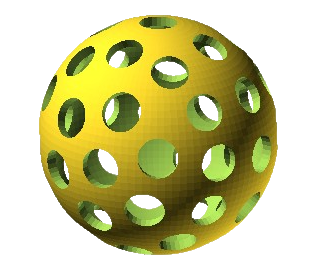
\includegraphics[width=0.25\linewidth]{images/image-removebg-preview.png}
    \caption{3D-printed spherical shell}
\end{figure}
The shell is mounted on a base that houses the battery along with all the previously mentioned components, including the microcontroller, audio amplifier module, signal generator, and remote-controlled switch. 
This base provides an organized and concealed arrangement of the internal components, offering the end user a polished and minimalist appearance while maintaining practicality.
\begin{figure}[H]
    \centering
    \begin{subfigure}[b]{0.4\linewidth}
        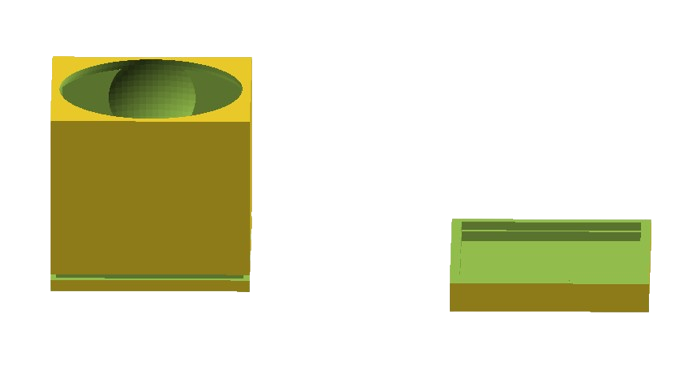
\includegraphics[width=\linewidth]{images/Supports.png}
        \caption{Support base}
    \end{subfigure}
    \begin{subfigure}[b]{0.4\linewidth}
        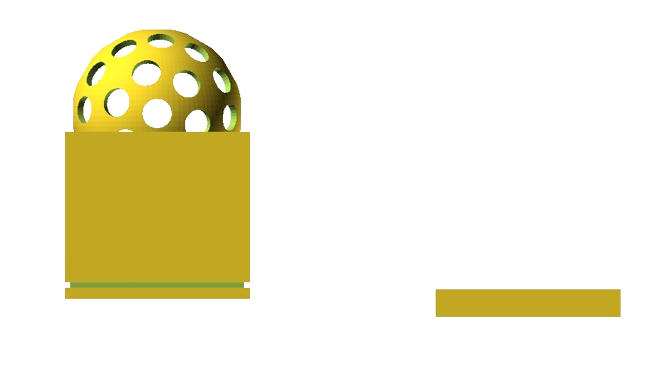
\includegraphics[width=\linewidth]{images/Jammer+Supports.png}
        \caption{Shell resting on the base}
    \end{subfigure}

\end{figure}
